\documentclass[aspectratio=43]{beamer}

\usepackage[utf8]{inputenc}
\usepackage[english]{babel}
\usepackage{csquotes}%Correctly typeset Vojtech
\usepackage{csvsimple}
\usepackage{booktabs}
\usepackage{styles/beamer_eit-en}
\usepackage{datetime2}
\usepackage[font={scriptsize}]{caption}%Smaller image captions, it for italics, can choose footnotesize to be even smaller
\captionsetup[figure]{labelformat=empty}%Remove "Figure" from the figure caption
%\setbeamertemplate{footline}[frame number]
%\setbeamerfont{footline}{series=\bfseries}

%Mathematic packages
\usepackage{amsmath}
\usepackage{amsbsy}

\usepackage[backend=biber, style=authoryear,]{biblatex}

% File is created and written to disk by the above package
\addbibresource{literature.bib}

\title[]{Algoritmo \textit{Array} e Filtro de Informação para Sistemas Lineares com Entradas Desconhecidas}

\author{Lucas Matos e Souza, Thiago Pereira Chagas, Gildson Queiroz de Jesus}

\institute{Programa de Pós-Graduação em Modelagem Computacional em\\
	Ciência e Tecnologia, Laboratório de Mecatrônica,\\
	UESC, Ilhéus, BA
}
\date[2019]{27/11/2019}%Put actual date of the presentation

\begin{document}

\begin{frame}
        \maketitle
\end{frame}

%\begin{frame}{Table of contents}
%        \tableofcontents
%\end{frame} ... its generally not necessery to provide table of contents for such short presentation

\section{Introdução}

\begin{frame}
	\frametitle{Introdução}
	\begin{itemize}
		\item A abordagem para estimação de estados em sistemas dinâmicos desenvolvida por Rudolf Kalman em \cite{Kalman1960} tem sido utilizada em diversos estudos na literatura.
		\item No decorrer da sua utilização algumas limitações foram apresentadas, pode-se exemplificar:
		\begin{itemize}
			\item problemas de convergência causados devido à falta de precisão dos algoritmos numéricos ou modelagem não apropriada dos sistemas a serem estimados \cite{Jesus2007};
			\item problema numérico na filtragem relacionado a condições iniciais desconhecidas do filtro Kalman.
		\end{itemize}
	\end{itemize}
\end{frame}

\begin{frame}
	\frametitle{Introdução}
	\begin{itemize}
		\item Na busca por soluções foram desenvolvidos novos algoritmos para diferentes implementações do filtro de Kalman, entre eles destacam-se a utilização de algoritmo \textit{array}, introduzido por Potter \cite{POTTER1963}, e o filtro na forma da informação \cite{Anderson1979}.
	\end{itemize}
\end{frame}
\section{Content}

\begin{frame}
	\frametitle{Sistemas Lineares com Entradas Desconhecidas - FKED}
	\begin{itemize}
		\item Em algumas aplicações de estimação de estados, surgem incertezas no sistema dinâmico, causados por pertubações que não podem ser medidas por depender de sensores de alto custo ou por complexidade de aplicação. Essas pertubações são denominadas de entradas desconhecidas.
		\item O problema em observar o vetor de estado de um sistema linear sujeito a entradas desconhecidas recebeu considerável atenção nas últimas 3 décadas \cite{Darouach1995, Hou1998, Hsieh2017, Li2018}. 
		\item Em \cite{Darouach1995}, foi apresentado um filtro para sistemas espaço de estado considerando a inclusão de entradas desconhecidas ou não mensuráveis em sua formulação.
	\end{itemize}
\end{frame}

\begin{frame}
	Considere o sistema dinâmico descrito por
	\begin{align}\label{eq:001}
		x_{k+1} &= Ax_{k} + Bu_{k} + Fd_{k} + w_{k}\nonumber \\
		y_{k} &= Hx_{k} + v_{k}, \quad \quad \quad \quad k \geq 0,
	\end{align}
	\begin{itemize}
		\item $x_{k} \in \mathbb{R}^{n}$ o vetor de estado, 
		\item $u_{k} \in \mathbb{R}^{m}$ o vetor de entrada de controle, \item $y_{k} \in \mathbb{R}^{p}$ a medida da saída, 
		\item $d_{k} \in \mathbb{R}^{q}$ a variável desconhecida.
		\item $A, B, F, H$ são as matrizes do sistema e tem dimensões apropriadas. 
		\item $w_{k} \in \mathbb{R}^{n}$ e $v_{k} \in \mathbb{R}^{p}$ as sequências de ruídos branco presentes no estado e na medida, suas covariâncias são dadas por $\textsc{E}(w_{k}w_{j}^{T}) = \textsc{W}\delta_{kj}$, $\textsc{E}(v_{k}v_{j}^{T}) = \textsc{V}\delta_{kj}$, $\textsc{W} > 0$ e $\textsc{V} > 0$ onde $\delta_{kj}$ é o delta de Kronecker.
	\end{itemize}
\end{frame}

\begin{frame}
	Suponha que:
	\begin{enumerate}
		\item $posto(H)=p$,
		\item $posto(F)=q$,
		\item $q\leq p$
		\item $posto(HF) = q$
	\end{enumerate}
	sejam satisfeitas, no \textbf{Algoritmo 1} temos o filtro de Kalman para sistemas lineares de tempo discreto com entradas desconhecidas fornecido em \cite{Darouach1995}.
\end{frame}

\begin{frame}
	\hline
	\vspace{0.1cm}
	\emph{\small \textbf{Algoritmo 1: FKED}}
	\vspace{0.1cm}
	\hline
	\vspace{0.1cm}
	\small \textit{\textbf{Passo $0$:}(Condições Iniciais): Se $P^{x}_{0} =  \phi$ então}
	\small 
	\begin{align}
		\bar{P}_{0} &= AP^{x}_{k|k}A^{T} + W \nonumber \\
		P^{d}_{0} &= \big(F^{T} H^{T} (V + H\bar{P}_{0} H^{T})^{-1} HF\big)^{-1} \label{eqPd} \nomumber \\
		P^{xd}_{1} &= P^{x}_{0} \bar{P}^{-1}_{0} F (F^{T} \bar{P}^{-1}_{0} F)^{-1} \nonumber \\
		P^{dx}_{1} &= P^{d}_{0} F^{T} \bar{P}^{-1}_{0} (\bar{P}^{-1}_{0} + H^{T} V^{-1} H)^{-1} \nonumber \\
		P^{x}_{1} &= (\bar{P}^{-1}_{0} + H^{T} V^{-1} H )^{-1} + P^{xd}_{1} (P^{d}_{0})^{-1} P^{dx}_{1}\label{eqPx} \nomumber
	\end{align}
	
	\small \textbf{Passo $1$:} \textit{Calcula a estimativa}
	\small
	\begin{align}
		\hat{x}_{k+1} &= \bar{x}_{k} + F\hat{d}_{k} + K_{k+1}^{x}\big(y_{k+1} - H(\bar{x}_{k} + F\hat{d}_{k})\big) \label{eqXhat}\nomumber \\
		\hat{d}_{k} &= K_{k+1}^{d}(y_{k+1} - H\hat{x}_{k}) \label{eqDhat}\nomumber \\
		\bar{x}_{k} &= A\hat{x}_{k} + Bu_{k} \nonumber
	\end{align}
	\small com, $K_{k+1}^{x} = (\bar{P}_{k}^{-1} + H^{T}V^{-1}H)^{-1}H^{T}V^{-1}$ e $K_{k+1}^{d} = P_{k+1}^{dx}H^{T}V^{-1}$.
	
	\vspace{0.2cm}
	\textbf{Passo $2$:} \textit{Atualizar os valores de $\bar{P}_{k|k}, P^{d}_{k}, P^{xd}_{k+1}, P^{dx}_{k+1}, P^{x}_{k+1}$.}
	\hline
\end{frame}

\begin{frame}
	\frametitle{FKED na forma da informação}
	\begin{itemize}
		\item O método do filtro na forma da informação, em síntese, expressa a estimativa ótima em torno do inverso da matriz de covariância do erro. Em determinadas circunstâncias, quando não há informações confiáveis sobre as condições iniciais do estado. No Algoritmo 2 é apresentado o FKED expresso na forma da informação.
	\end{itemize}
\end{frame}

\begin{frame}
	\hline
		\small	\emph{\textbf{Algoritmo 2: FKED na forma da Informação}}
	\hline
	\vspace{0.1cm}
	\small \textbf{Passo $0$:} \textit{(Condições Iniciais): Se $(P^{x}_{0})^{-1} =  \phi^{-1}$ então}
	\small
	\begin{align}
		\bar{P}_{0} &= AP^{x}_{0}A^{T} + W \nonumber \\
		P^{d}_{0} &= \big(F^{T} H^{T} (V + H\bar{P}_{0} H^{T})^{-1} HF\big)^{-1} \nonumber \\
		P^{xd}_{0} &= P^{x}_{1} \bar{P}^{-1}_{0} F (F^{T} \bar{P}^{-1}_{0} F)^{-1} \nonumber \\
		P^{dx}_{0} &= P^{d}_{0} F^{T} \bar{P}^{-1}_{0} (\bar{P}^{-1}_{0} + H^{T} V^{-1} H)^{-1} \nonumber
	\end{align}

	\small \textbf{Passo $1$:} \textit{Calcular os valores de $\big(P^{x}_{k+1}\big)^{-1}$ e $(P^{x}_{k+1})^{-1}\hat{x}_{K+1} = o_{k}$:}
	\small{
	\begin{align}
		\big(P^{x}_{k+1}\big)^{-1} &=\bigg(\bigg(\bar{\bar{P}} + H^{T} V^{-1} H \bigg)^{-1} + P^{xd}_{k+1} (P^{d}_{k})^{-1} P^{dx}_{k+1} \bigg)^{-1}\\
		(P^{x}_{k+1})^{-1}\hat{x}_{K+1} &= (P^{x}_{k+1})^{-1}\big( \bar{\bar{x}}_{k} + F\hat{\hat{d}}_{k} + K^{x}_{k+1} \big( y_{k+1} - H ( \bar{\bar{x}} + F \hat{\hat{d}}_{k} ) \big) \big) = o_{k}
	\end{align}}
	\hline
\end{frame}

\begin{frame}
	\hline
	\small	\emph{\textbf{Algoritmo 2: FKED na forma da Informação - Continuação}}
	\hline
	\vspace{0.1cm}
	\small Quando,
	\begin{align}
		\bar{\bar{P}}_{k} &= W^{-1} - W^{-1}A\big((P^{x}_{k})^{-1} + A^{T}W^{-1}A \big)^{-1}A^{T}W^{-1}\nonumber \\
		\bar{\bar{x}}_{k} &= AP^{x}_{k}(P^{x}_{k})^{-1}\hat{x}_{k} + Bu_{k}\nonumber \\
		\hat{\hat{d}}_{k} &= K^{d}_{k+1}y_{k+1} - K^{d}_{k+1}H\bar{\bar{x}}_{k}\\
		K_{k+1}^{x} &= (\bar{P}_{k|k}^{-1} + H^{T}V^{-1}H)^{-1}H^{T}V^{-1}\nonumber \\
		K_{k+1}^{d} &= P_{k+1|k+1}^{dx}H^{T}V^{-1} \nonumber
	\end{align}
	
	\small \textbf{Passo $2$:} \textit{Atualizar os valores de $\big(P^{x}_{k+1}\big)^{-1}$ e $(P^{x}_{k+1})^{-1}\hat{x}_{K+1} = o_{k}$.}
	\hline
\end{frame}

\begin{frame}
	\frametitle{Algoritmo \textit{array} para FKED}
	\begin{itemize}
		\item A seguir, no Algoritmo 3, é mostrado o método do algoritmo \textit{array} para o FKED. Este aumenta a eficiência e estabilidade numérica nas implementações dos filtros devido ao uso de transformações ortogonais nos cálculos, o que o torna mais estável numericamente se comparado às equações \eqref{eqPd} e \eqref{eqPx} que estão na forma de Riccati e são utilizadas nas implementações dos filtros de Kalman.
	\end{itemize}
\end{frame}

\begin{frame}
	\hline
	\small \emph{\textbf{Algoritmo 3: Algoritmo \textit{array }para FKED}}
	\hline
	\small \textbf{Passo $0$:} \textit{(Condições Iniciais): Se $(P^{x}_{0})^{1/2} = (\Psi)^{1/2}$ então}
	\small
	\begin{align*}
		\bar{P}_{0} = AP^{x}_{0}A^{T} + W		
	\end{align*}
	
	\small \textbf{Passo $1$:} \textit{Calcular $\big( P^{d}_{k} \big)$,utilizando uma matriz unitária $\Phi$ tal que:}
	\small
	\begin{align}
		\begin{bmatrix}
			\bar{P}_{k}^{-1/2} & H^{T}V^{-1/2}
			\\
			0 & F^{T}H^{T}V^{-1/2}
		\end{bmatrix}\Phi
		=
		\begin{bmatrix}
			\mathcal{E}^{1/2} & 0
			\\
			\big( F^{T}H^{T}V^{-1}H \big) \mathcal{E}^{-1/2} & \big( P^{d}_{k}\big)^{-1/2}
		\end{bmatrix}
	\end{align}
	\small sendo $\mathcal{E} = \bar P_{k}^{ - 1} + {H^T}{V^{ - 1}}H$.
	
	\small \textbf{Passo $2$:} \textit{ Atualizar o valor de $P^{xd}, P^{dx}$:}
	\small
	\begin{align}
		P^{xd}_{k+1} &= P^{x}_{0} \bar{P}^{-1}_{0} F (F^{T} \bar{P}^{-1}_{0} F)^{-1} \nonumber\\
		P^{dx}_{k+1} &= P^{d}_{k} F^{T} \bar{P}^{-1}_{0} (\bar{P}^{-1}_{0} + H^{T} V^{-1} H)^{-1}
	\end{align}
	\hline
\end{frame}

\begin{frame}
	\hline
	\small \emph{\textbf{Algoritmo 3: Algoritmo \textit{array }para FKED - Continuação}}
	\hline
	\small \textbf{Passo $3$:} \textit{Calcular $\big(P^{x}_{k+1}\big)^{1/2}$, utilizando uma matriz unitária $\Theta$ tal que:}
	\small
	\begin{align}
		\begin{bmatrix}
			V^{1/2} & H W^{1/2} & H A \left( P_{k}^{x} \right)^{1/2} & 0
			\\ 
			0 & W^{1/2} & A \left( P_{k}^{x} \right)^{1/2} & P_{k+1}^{xd} (P_{k}^{d})^{-1/2}
		\end{bmatrix} \Theta
		=\nonumber \\
		\begin{bmatrix}
			\Pi^{1/2} & 0 & 0 & 0
			\\
			\left( W H^{T} + A P_{k}^{x} A^{T} H^{T} \right) \Pi^{-1/2} & \left( P^{x}_{k+1} \right)^{1/2} & 0 & 0
		\end{bmatrix}
	\end{align}
	\smallsendo $ \Pi = V + H W + H A P_{k}^{x} A^{T} H^{T}$.
	
	\small \textbf{Passo $4$:} \textit{Atualizar os valores de $\bar{P}_{k}$.}
	\hline
\end{frame}

\begin{frame}
	\frametitle{Exemplo Numérico}
	Considere o sistema linear com entradas desconhecidas modeladas de acordo com as equações \eqref{eq:001}, cujas matrizes são dadas por:
	\begin{align*}\label{matrizesExemplos}
		A = \begin{bmatrix} 0 & 0.6\\ 0.75 & 0 \end{bmatrix};
		B = \begin{bmatrix}  1 \\ 1\end{bmatrix};
		F = \begin{bmatrix}  1 \\ 1\end{bmatrix};
		H = \begin{bmatrix}  1 & 1\\ 0 & 1\end{bmatrix};
	\end{align*}
	$w_{k} \in \mathbb{R}^{n}$ e $v_{k} \in \mathbb{R}^{p}$ as sequências de ruídos branco presentes no estado e na medida, estes ruídos não possuem correlação com o estado inicial do sistema, suas matrizes de covariâncias $V, W$ são:
	$V = \begin{bmatrix}  12 & 0\\ 0 & 12 \end{bmatrix}$ e $W = \begin{bmatrix}  3 & 0\\ 0 & 6 \end{bmatrix}$. A previsão inicial do estado e da entrada desconhecida é assumida como zero e sua informação estatística é dada por:$P^{x}_{0} = \begin{bmatrix}  1 & 0\\ 0 & 1 \end{bmatrix}$.
\end{frame}

\begin{frame}
	\begin{figure}
		\centering
		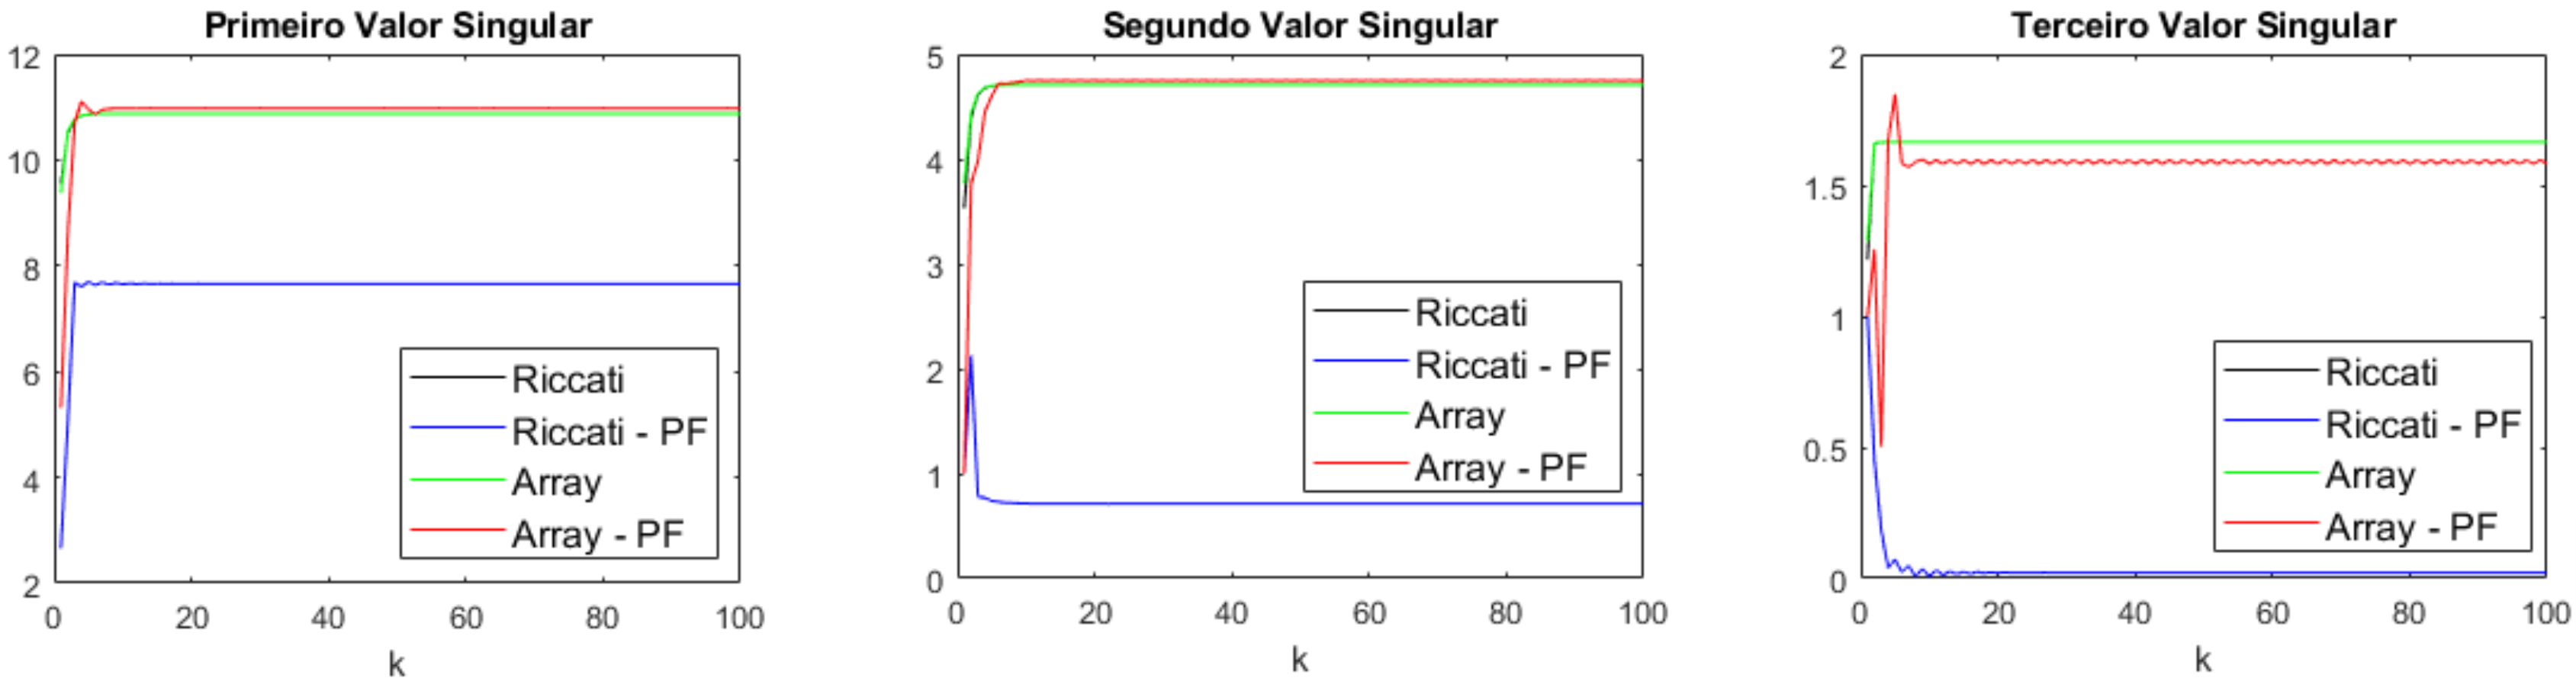
\includegraphics[width=1.05\textwidth]{figuras/valores-singular-color}
		\caption{Valores singulares de $P_{k}$ simulação do algoritmo \textit{array}}
		\label{fig:singular-array}
	\end{figure}
\end{frame}

\begin{frame}
	\begin{figure}
		\centering
		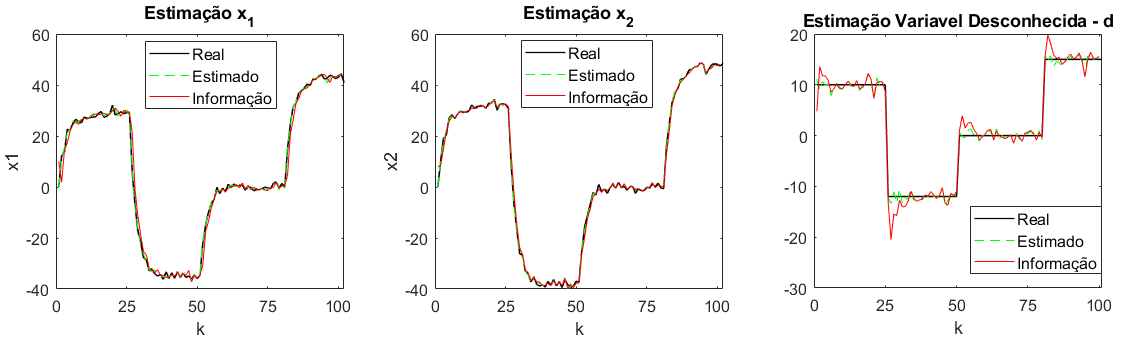
\includegraphics[width=1.05\textwidth]{figuras/estimacoes-info-color}
		\caption{Estimação do estado e da variável desconhecida - simulação do Filtro na forma de informação}
		\label{fig:estimacao-info}
	\end{figure}
\end{frame}

\begin{frame}
	\begin{figure}
		\centering
		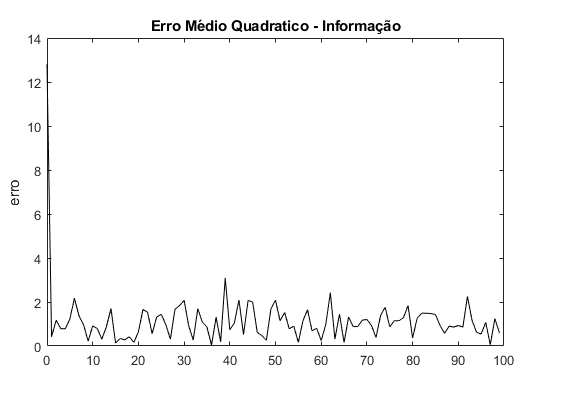
\includegraphics[width=0.5\textwidth]{figuras/erro-comparacao-informacao}
		\caption{Erro médio quadrático - Filtro na forma de informação}
		\label{fig:erro-info}
	\end{figure}
\end{frame}
\section{Summary}
\begin{frame}{Summary}
    \begin{itemize}
        \item Don't forget to put in the summary.
        \item Try to reduce LaTeX warnings number.
        \item Resolve any LaTeX errors.
    \end{itemize}
\end{frame}

\begin{frame}[t,allowframebreaks]
  \frametitle{Literature}
  \printbibliography
 \end{frame}

\end{document}
